% --------------------------
% Document class
% --------------------------
\documentclass[
A4paper,                % paper size A4
twoside,                % onesite or twoside printing
openright,              % doublepage cleaning ends up right side
chapterprefix=true,     % prefix for chapter marks
12pt,                   % font size
headings=normal,        % size of headings
titlepage=on            % own page for each title page
]{book}

% **************************************************
% THESIS details
% **************************************************

\newcommand{\University}{\protect{Universidad Polit\'ecnica de Madrid}}
\newcommand{\UNIVERSITY}{\protect{UNIVERSIDAD POLIT\'ECNICA DE MADRID}}

% **************************************************
% THESIS COVER DATA
% **************************************************
% Rellena aquí los datos de la portada.
% NOTA: completar los apellidos de la directora cuando se confirmen.

\newcommand{\thesisTitle}{\protect {Aprendizaje profundo aplicado a la microestructura de mercados de predicción: predicción de corto plazo en mercados de Bitcoin de Polymarket}}
\newcommand{\thesisAuthor}{\protect{Marc Maldonado Lorca}}

\newcommand{\thesisDate}{2026}

\newcommand{\UPMCentre}{\protect {Escuela Técnica Superior de Ingeniería de Sistemas Informáticos}}


\newcommand{\DoctoralProgramme}{\protect{Máster de Formación Permanente en Deep Learning}}

\newcommand{\supervisor}{Dra. Inmaculada <Apellidos>}
\newcommand{\cosupervisor}{}

\newcommand{\supervisorDetails}{Dra. Inmaculada <Apellidos>, <puesto>, Universidad Politécnica de Madrid}
\newcommand{\cosupervisorDetails}{}


% **************************************************
% Settings
% **************************************************

% **************************************************
% Settings
% **************************************************
% --------------------------
% Packages
% --------------------------
\usepackage[spanish,english,es-tabla,es-noshorthands]{babel}  % es-noshorthands: evita que < > " activen atajos (conflicto con TikZ)
\usepackage{iftex}
\ifPDFTeX
  \usepackage[utf8]{inputenc}   % solo pdfLaTeX: XeTeX/LuaTeX (tectonic) ya leen UTF-8 nativo
  \usepackage[T1]{fontenc}      % cargar inputenc bajo XeTeX corrompe ¿ ¡ — por eso se condiciona
\fi
\usepackage{lmodern}     % Use a modern font (that is not pixelated)
\usepackage[protrusion=true, expansion=false]{microtype}  % expansion=false: compatible con XeTeX/tectonic
\usepackage{amsmath,amssymb} 
\usepackage{tabularx}    % tables spanning the full text width
\usepackage{multicol}    % multi-columns in tables
\usepackage{multirow}    % multi-rows in tables
\usepackage{longtable}   % tables spanning more than one page
\usepackage{booktabs}    % nicer horizontal rules in tables
\usepackage{ltablex}
\usepackage{setspace}
\usepackage{tikz}                % drawing custom shapes
\usetikzlibrary{positioning,arrows.meta,calc,fit,backgrounds}  % librerías usadas en los diagramas
\usepackage{graphicx,graphics}   % packages to manage images
% \usepackage{subfigure}         % (obsoleto; en conflicto con subcaption, usado abajo)
\usepackage[export]{adjustbox}
\usepackage{ragged2e} 
\usepackage{comment} 
\usepackage{blindtext}
\usepackage[acronym,nonumberlist,nomain]{glossaries}  % package for list of acronyms
\usepackage{hyperref}
\usepackage{geometry}
\usepackage{parskip}     % paragraph spacing (suppress indentation)
\usepackage{fancyhdr}    % personalizar encabezado
\usepackage{enumitem}
\usepackage{xcolor}
\usepackage{emptypage}   % no headers in empty pages
\usepackage[small,hang,bf]{caption}    % caption options
\usepackage{subcaption}   

%%% BIBLIOGRAPHY
% The style used is APA. A list of available styles is available  at https://www.overleaf.com/learn/latex/Biblatex_bibliography_styles

% NOTA (tooling): la plantilla oficial usa biblatex+biber con estilo APA. En este
% entorno se compila con tectonic, que no incluye biber, por lo que la bibliografía
% se gestiona de forma manual (mainmatter/references.tex) y este bloque queda
% desactivado. Para recuperar la bibliografía APA oficial (p. ej. compilando en
% Overleaf, que sí trae biber), descomenta este bloque y \printbibliography en main.tex.
%
% \usepackage[
% backend=biber,
% style=apa,
% sorting=nyt,
% doi=true,
% url=false,
% isbn=false,
% backref=false
% ]{biblatex}
%
% \addbibresource{thesisRefs.bib}

% --------------------------
% Customize document
% --------------------------
% Define the geometry and the physical page size.  \newgeometry would reset the
% paper stock to the engine default (US Letter), so the setting belongs here.
\geometry{a4paper, top=2.5cm, bottom=2.5cm, right=2.5cm, left=2.5cm}

\setlength{\parskip}{10pt}   % Change the default value

% hiperlinks
\hypersetup{
    colorlinks=true,          % Enable colored links
    linkcolor=black,          % Color for internal links
    urlcolor=blue,
    citecolor=blue
}

% Header and footer
\fancyhf{}   % Clear the default header and footer
\renewcommand{\headrulewidth}{0.2pt}
\setlength{\headheight}{14.5pt}
\fancyhead[R]{\nouppercase{\leftmark}}
\fancyfoot[C]{\thepage}

\addto\captionsspanish{\renewcommand{\contentsname}{Tabla de Contenido}}
\addto\captionsspanish{\renewcommand{\listfigurename}{Lista de Figuras}}
\addto\captionsspanish{\renewcommand{\listtablename}{Lista de Tablas}}

% Increase indentation in lists
\newlist{mydescription}{description}{1}
\setlist[mydescription,1]{labelindent=2em, leftmargin=2em}


% **************************************************
% Begin document
% **************************************************
\begin{document}

% --------------------------
% Cover and front matter
% --------------------------
\frontmatter
\pagestyle{empty}				    % no header nor footer
% called by main.tex
\begin{titlepage}
\begin{center}
\begin{spacing}{1.3}
    \textbf{\large {\UNIVERSITY}}\\
    \textbf{\large {\UPMCentre}}\\
    \vspace{5mm}
\end{spacing}

\begin{minipage}[c]{0.45\textwidth}
    \centering
    
\includegraphics[width=6cm]{figures/EscudoUPM.png}
\end{minipage}
\hfill
\begin{minipage}[c]{0.45\textwidth}
    \centering
    
\includegraphics[width=6cm]{figures/logo_master_v2.pdf}
\end{minipage}

\vspace{8mm}

\begin{spacing}{1.55}
\textbf{\LARGE {\thesisTitle}}
\end{spacing}

\vspace{8mm}

\begin{spacing}{1.15}
\textbf{\LARGE {MÁSTER DE FORMACIÓN PERMANENTE}}\\
\vspace{3mm}
\textbf{\LARGE {EN DEEP LEARNING}}\\
\vspace{8mm}

\medskip
{\large {Presentado por:}}
\end{spacing}
\end{center}





\begin{center}
\begin{spacing}{0.8}
\textbf{\Large {\thesisAuthor}}\\
\end{spacing}
\end{center}



\vspace{3mm}
\begin{center}
\begin{spacing}{1.3}
{Bajo la dirección de:}\\
    {\large {\supervisor}}\\
    {\large {\cosupervisor }}
\end{spacing}
\end{center}

\vspace{\fill}

\begin{center}
    \large {Madrid, \thesisDate}
\end{center}
\end{titlepage}

\newpage



\pagenumbering{roman}			    % roman page numbering 
\pagestyle{plain}				    % empty header, just page number in footer
% called by main.tex

\begin{spacing}{1.3}
Título: \thesisTitle \\
Autor: \thesisAuthor\\
Máster de Formación Permanente en Deep Learning\\
Universidad Politécnica de Madrid\end{spacing}
Dirección de Tesis: 
\begin{mydescription}
    \item \supervisorDetails  (Directora)
    \item \cosupervisorDetails
\end{mydescription}

\vspace{10 mm}
%Revisores Externos: <borrar este texto para dejar este apartado en blanco>

\vspace{30 mm}

Tribunal: <borrar este texto para dejar este apartado en blanco>


\vspace{50mm}



Fecha de Defensa del TFM: <borrar este texto para dejar este apartado en blanco>



\vspace{\fill}
% \begin{spacing}{1.0}
% < Si el trabajo ha recibido financiación de alguna convocatoria competitiva, hacerlo constar aquí  escribiendo: “Esta tesis ha sido parcialmente financiada por....” En caso contrario,  borrar este texto para dejar este apartado en blanco. >
% \end{spacing}


\cleardoublepage

% called by main.tex
%


\vspace*{\fill}
\begin{flushright} 
    \textit{}% Dedicatoria (opcional): rellenar si se desea.
    \vspace{15cm}
\end{flushright}
   % dedication (optional)
\cleardoublepage

% called by main.tex
%
\section*{Agradecimientos}
\label{sec::agradecimientos}
\addcontentsline{toc}{section}{Agradecimientos}


Quiero agradecer especialmente a mi amigo Ramón, que me introdujo en este mundo y sin cuya
curiosidad inicial este trabajo no habría existido. Gracias también a mi directora por su
guía a lo largo del proyecto, y a mi familia y amigos por su apoyo durante el máster.





  % acknowledgement (optional)
\newpage

% called by main.tex
%

\section*{Abstract}
\addcontentsline{toc}{section}{Abstract}
\label{sec::abstract}

This work studies whether deep learning can exploit market microstructure signals to
anticipate the short-term price movement of binary contracts on Bitcoin traded on
Polymarket, a prediction market. Unlike the literature focused on how the event finally
resolves, here we target the local movements of the contract price over windows of a few
seconds, combining the order book with external Bitcoin market references (spot, perpetual
futures and a price oracle). The main contribution is not a single model but a
reproducible methodology: a multi-source data capture system with per-session quality
control, strictly temporal validation, and an evaluation that incorporates realistic
execution costs and latency. The central, uncomfortable finding is that a directional
classifier that is correct nearly nine out of ten times stops being profitable once a
realistic two-second entry latency is introduced: what decides the outcome is cost and
execution, not directional accuracy. Building on this, we evaluate a progression of models
(tabular baselines, latency-aware models, and sequential and convolutional architectures
over the order book) and a frozen tabular specialist. On the untouched five-day
out-of-sample block, the specialist obtains a modest positive mean at the reference cost
(+0.349 ticks per action, 754 actions and three out of five positive days), but turns
slightly negative under the full-cost stress test. A volatility filter, whose numerical
threshold came from the training period, is then explored after detecting a regime shift;
it improves the result on the same block, so it is reported as a post-hoc diagnostic rather
than as confirmatory evidence. We report every figure in net ticks together with its support
and uncertainty, and we do not claim real profitability: the deliverable is the
methodology, the evidence obtained under an auditable protocol, and the explicit
delimitation of its limits.

\newpage
\section*{Resumen}
\addcontentsline{toc}{section}{Resumen}
\label{sec::resumen}

Este trabajo estudia si el aprendizaje profundo puede aprovechar señales de
microestructura de mercado para anticipar el movimiento de corto plazo del precio de los
contratos binarios sobre Bitcoin negociados en Polymarket, un mercado de predicción. A
diferencia de la literatura centrada en cómo se resuelve finalmente el evento, aquí el
objetivo son los movimientos locales del precio del contrato en ventanas de pocos
segundos, combinando el libro de órdenes con referencias externas del mercado de Bitcoin
(contado, futuros perpetuos y un oráculo de precios). La aportación principal no es un
modelo concreto, sino una metodología reproducible: un sistema de captura de datos
multifuente con control de calidad por sesión, una validación estrictamente temporal y una
evaluación que incorpora costes de ejecución y latencia realistas. El hallazgo central, y
algo incómodo, es que un clasificador direccional que acierta casi nueve de cada diez veces
deja de ser rentable en cuanto se introduce una latencia de entrada realista de dos
segundos: lo que decide el resultado es el coste y la ejecución, no el acierto direccional.
A partir de ahí se evalúa una progresión de modelos (líneas base tabulares, modelos
sensibles a la latencia y arquitecturas secuenciales y convolucionales sobre el libro de
órdenes) y un especialista tabular congelado. En el bloque intacto de cinco días fuera de
muestra, el especialista obtiene un promedio modestamente positivo al coste de referencia
($+0{,}349$ ticks por acción, 754 acciones y tres de cinco días positivos), pero pasa a ser
ligeramente negativo bajo el coste de estrés completo. Tras detectar un cambio de régimen se
explora un filtro de volatilidad cuyo umbral numérico procede del entrenamiento; como la
decisión de incorporarlo se evalúa sobre ese mismo bloque, su mejora se presenta como
diagnóstico \emph{post-hoc}, no como evidencia confirmatoria. Todos los resultados se reportan
en ticks netos junto a su soporte e incertidumbre, y no se afirma rentabilidad real: lo que
se entrega es la metodología, la evidencia obtenida bajo un protocolo auditable y la
delimitación explícita de sus límites.
		% abstract (in English and Spanish)
\newpage

\selectlanguage{spanish}

\setcounter{tocdepth}{3}		% define depth of toc
\tableofcontents				% display table of contents


\addcontentsline{toc}{section}{Lista de Figuras}
\listoffigures


\addcontentsline{toc}{section}{Lista de Tablas}
\listoftables
\newpage

% called by main.tex
%
\section*{Abreviaturas y acrónimos}
\addcontentsline{toc}{section}{Abreviaturas y acrónimos}
\label{sec::acronimos}

\vspace{10 mm}
\begin{description}[align=right,labelwidth=2.5cm]
\item [UPM] Universidad Politécnica de Madrid
\item [TFM] Trabajo Fin de Máster
\item [LOB] Libro de órdenes (\textit{Limit Order Book})
\item [BTC] Bitcoin
\item [AUC] Área bajo la curva ROC (\textit{Area Under the Curve})
\item [EV] Valor esperado (\textit{Expected Value})
\item [HGB] \textit{Histogram-based Gradient Boosting}
\item [GRU] Unidad recurrente con puertas (\textit{Gated Recurrent Unit})
\item [LSTM] Memoria larga a corto plazo (\textit{Long Short-Term Memory})
\item [CNN] Red neuronal convolucional (\textit{Convolutional Neural Network})
\item [TCN] Red convolucional temporal (\textit{Temporal Convolutional Network})
\item [OOF] Fuera de pliegue (\textit{Out-Of-Fold})
\item [OOS] Fuera de muestra (\textit{Out-Of-Sample})
\item [IC] Intervalo de confianza
\item [QA] Control de calidad (\textit{Quality Assurance})
\item [API] Interfaz de programación de aplicaciones (\textit{Application Programming Interface})
\item [bps] Puntos básicos (\textit{basis points})
\end{description}

\cleardoublepage

% --------------------------
% Main matter
% --------------------------
\mainmatter
\pagenumbering{arabic}			% arabic page numbering
\setcounter{page}{1}			% set page counter
\pagestyle{fancy} 	            % fancy header and footer
\parskip=7pt                    % space after each paragraph
\parindent=0pt                  % suppress indentation of paragraphs


% Capítulos
% called by main.tex
%
\chapter{Introducción}
\label{ch::introduccion}

Este Trabajo Fin de Máster estudia un problema de predicción financiera de muy corto
plazo en un entorno poco habitual: los mercados de predicción sobre el precio de Bitcoin
de la plataforma Polymarket. El objetivo no es un sistema de trading en producción, sino
una \emph{metodología} rigurosa para responder, con honestidad estadística, a una
pregunta concreta: ¿contiene el libro de órdenes de estos mercados señales que permitan
anticipar el movimiento del precio en los próximos segundos y que, además, sobrevivan a
los costes y a la latencia reales de operar?

Como el lector puede no estar familiarizado con el mundo de las criptomonedas ni con la
microestructura de mercado, este capítulo introduce todos los conceptos desde cero antes
de plantear el problema y los objetivos.

\section{Introducción y definición del problema}

Esta sección define el problema desde cero. Antes de plantear la pregunta de
investigación se introducen los conceptos imprescindibles —mercado de predicción,
contrato binario, libro de órdenes y señales de microestructura—, de modo que el documento
resulte autocontenido también para un lector ajeno al mundo de las criptomonedas. Con ese
vocabulario fijado, se enuncia el problema concreto que se aborda.

\subsection{Qué es un mercado de predicción}

Un \emph{mercado de predicción} es un mercado en el que se compran y venden contratos
cuyo valor depende del resultado de un acontecimiento futuro. El caso más sencillo es el
\emph{contrato binario}: un contrato que pagará una unidad monetaria si el acontecimiento
ocurre y cero si no ocurre. Por construcción, su precio se mueve entre 0 y 1, y puede
leerse directamente como la \emph{probabilidad implícita} que el mercado asigna al
suceso. Por ejemplo, un contrato ``el precio de Bitcoin estará por encima de un umbral a
una hora determinada'' que cotiza a 0,60 indica que el mercado estima una probabilidad
cercana al 60\,\% de que eso ocurra. Cuando el acontecimiento se resuelve, el contrato
vale 1 o 0 y las posiciones se liquidan. La literatura clásica ha mostrado que estos
mercados agregan información dispersa y producen previsiones razonablemente
calibradas~\cite{wolfers2004prediction}.

\subsection{Qué es Polymarket}

Polymarket es una plataforma de mercados de predicción descentralizada. A diferencia de
una casa de apuestas, donde el operador fija las cuotas, en Polymarket son los propios
participantes quienes ponen precios mediante un \emph{libro de órdenes}: el emparejamiento
de compras y ventas ocurre fuera de la cadena de bloques (de forma rápida) y la
liquidación final del dinero se registra en cadena (sobre una \emph{blockchain})
\cite{polymarket_trading}. En los mercados sobre el precio de Bitcoin, cada contrato
binario toma valores entre 0 y 1 y se interpreta como una
probabilidad~\cite{polymarket_prices}. Esto convierte cada mercado en un pequeño
\emph{mercado electrónico} (\emph{exchange}) con su propia dinámica de oferta y demanda.

\subsection{El libro de órdenes y el vocabulario de la microestructura}

El \emph{libro de órdenes} (en inglés \emph{limit order book}, LOB) es la lista, ordenada
por precio, de todas las órdenes de compra y de venta que están a la espera de ejecutarse.
Sus elementos esenciales son:

\begin{itemize}
  \item \textbf{Bid}: el precio más alto al que alguien está dispuesto a comprar.
  \item \textbf{Ask}: el precio más bajo al que alguien está dispuesto a vender. Siempre
  es mayor o igual que el \emph{bid}.
  \item \textbf{Spread}: la diferencia entre el \emph{ask} y el \emph{bid}. Es el primer
  coste de operar: quien compra al \emph{ask} y vende al \emph{bid} pierde el \emph{spread}.
  \item \textbf{Profundidad}: el volumen disponible en cada nivel de precio. A más
  profundidad, más se puede operar sin mover el precio.
  \item \textbf{Precio medio} (\emph{mid}): el punto medio entre \emph{bid} y \emph{ask};
  una referencia ``limpia'' del precio sin el ruido del \emph{spread}.
  \item \textbf{Tick}: la variación mínima de precio que admite el mercado. Es la unidad
  natural en la que mediremos todos los resultados de este trabajo.
\end{itemize}

La \emph{microestructura de mercado} es la rama que estudia cómo se forman los precios a
partir de estos mecanismos —órdenes, \emph{spread}, profundidad y flujo de
operaciones— a escalas de tiempo muy finas. La Figura~\ref{fig:mercado} resume el entorno:
el precio del contrato se forma en su propio libro de órdenes, pero está acoplado a
referencias externas del mercado de Bitcoin (mercado al contado, futuros perpetuos y un
oráculo de precios), porque al fin y al cabo el contrato habla del precio de Bitcoin.

\begin{figure}[h]
\centering
\begin{tikzpicture}[
  node distance=8mm,
  box/.style={draw, rounded corners, align=center, minimum height=9mm, inner sep=4pt, font=\small},
  ext/.style={box, fill=blue!6},
  core/.style={box, fill=orange!12, thick},
  tgt/.style={box, fill=green!10},
  >=latex
]
\node[ext] (spot) {Mercado al contado\\(spot BTC)};
\node[ext, below=of spot] (perp) {Futuros perpetuos\\(perp BTC)};
\node[ext, below=of perp] (oracle) {Oráculo de precios};
\node[core, right=22mm of perp] (lob) {Libro de órdenes\\del contrato\\(\emph{bid}, \emph{ask}, \emph{spread})};
\node[tgt, right=22mm of lob] (mid) {Precio del contrato\\$m_t \in [0,1]$};
\node[box, below=14mm of mid, fill=gray!8] (pred) {Pregunta: ¿hacia dónde\\se mueve $m_t$ en los\\próximos segundos?};
\draw[->] (spot) -- (lob);
\draw[->] (perp) -- (lob);
\draw[->] (oracle) -- (lob);
\draw[->] (lob) -- (mid);
\draw[->] (mid) -- (pred);
\end{tikzpicture}
\caption{El entorno del problema. El precio del contrato binario se forma en su libro de
órdenes y está acoplado a referencias externas del mercado de Bitcoin. El objetivo es
anticipar su movimiento de muy corto plazo.}
\label{fig:mercado}
\end{figure}

\subsection{Definición del problema}

El precio del contrato no es el precio de Bitcoin: es una función no lineal y dependiente
del tiempo de la probabilidad de que el suceso se resuelva afirmativamente. Sin embargo,
está acoplado a las referencias externas observables que se acaban de citar. Un modelo
útil debe, por tanto, aprender dos cosas a la vez: la dinámica interna del libro de
órdenes y la semántica del contrato respecto a Bitcoin.

El problema que se aborda es de microestructura y de muy corto plazo: dado el estado del
mercado en un instante $t$ (libro de órdenes y referencias externas), predecir el
movimiento del precio medio del contrato en una ventana de pocas decenas de segundos. A
diferencia de la mayor parte de la literatura sobre mercados de predicción, que estudia
cómo se calibra el precio frente a la resolución final del evento, aquí el interés está en
los movimientos locales del precio, a escala de segundos.

Conviene fijar desde el principio un matiz que vertebra todo el trabajo: una buena
capacidad de \emph{predecir la dirección} no implica una estrategia rentable. Una métrica
de clasificación puede ser muy alta y, aun así, el sistema no ser explotable si opera con
retraso, si aprende artefactos del propio conjunto de datos o si ignora el coste real de
cruzar una orden. Por eso el problema no se evalúa por el acierto, sino por el resultado
económico neto, una vez descontados costes y latencia realistas.

\section{Motivación}

La motivación de este trabajo es doble. Desde el punto de vista aplicado, los mercados de
predicción de criptoactivos son un entorno joven, con menos competencia algorítmica que
los mercados financieros tradicionales, y con datos públicos accesibles; resulta natural
preguntarse si contienen señales explotables. Desde el punto de vista metodológico —que es
el que da peso a una memoria de máster— el entorno es un excelente banco de pruebas para
una cuestión central en el aprendizaje automático aplicado a finanzas: la distancia entre
\emph{predecir bien} y \emph{ganar dinero}.

Esa distancia es el hilo conductor. Como se mostrará, un clasificador direccional sencillo
alcanza una precisión cercana al 90\,\% y, pese a ello, deja de ser rentable en cuanto se
introduce una latencia de entrada realista de dos segundos. El coste y la ejecución, y no
el acierto, determinan el resultado. Asumir lo contrario es uno de los errores más comunes
y costosos en este campo, y documentarlo con evidencia cuantitativa es, en sí mismo, una
aportación.

\section{Objetivos}

El objetivo general es \textbf{construir y validar, con un protocolo honesto, una
metodología completa para evaluar si el aprendizaje automático y profundo pueden anticipar
el movimiento de corto plazo del precio de los contratos de Bitcoin de Polymarket bajo
costes y latencia realistas}. De él se derivan los siguientes objetivos específicos:

\begin{enumerate}[noitemsep]
  \item Diseñar un sistema de captura de datos multifuente, con control de calidad por
  sesión, que produzca un corpus alineado temporalmente y libre de fugas.
  \item Definir un protocolo de evaluación que combine validación estrictamente temporal,
  un modelo explícito de costes y una latencia medida empíricamente.
  \item Cuantificar el impacto de la latencia sobre una señal direccional fuerte, para
  delimitar dónde se rompe la cadena entre predicción y ejecución.
  \item Evaluar una progresión de modelos, de menor a mayor complejidad (líneas base
  tabulares, modelos sensibles a la latencia y arquitecturas profundas sobre el libro de
  órdenes), exigiendo que cada incremento de complejidad se justifique con evidencia.
  \item Determinar si existe un candidato que sobreviva a una validación fuera de muestra
  bajo coste, y delimitar con rigor sus límites y su incertidumbre.
\end{enumerate}

El presente trabajo se organiza como sigue. El Capítulo~\ref{ch::estado} revisa el estado
de la cuestión. El Capítulo~\ref{ch::metodos} describe los datos, las líneas base y la
metodología de modelado y entrenamiento. El Capítulo~\ref{ch::resultados} presenta y
analiza los resultados sobre el conjunto fuera de muestra. El Capítulo~\ref{ch::despliegue}
discute la estrategia de despliegue. El Capítulo~\ref{ch::etica} aborda los aspectos éticos
y las limitaciones. El Capítulo~\ref{ch::reproducibilidad} detalla la reproducibilidad, y
el Capítulo~\ref{ch::conclusiones} recoge las conclusiones. Por último, los anexos incluyen
un glosario de términos para el lector no familiarizado con las criptomonedas, el detalle de
las características y los hiperparámetros de los modelos.

% called by main.tex
%
\chapter{Estado de la cuestión}
\label{ch::estado}

Este capítulo sitúa el trabajo en la literatura. Se organiza en cinco áreas que confluyen
en el problema —mercados de predicción, aprendizaje profundo sobre libros de órdenes,
microestructura y ejecución, validación temporal en finanzas, y cambio de
distribución— y termina señalando el hueco concreto que este trabajo pretende cubrir.

\section{Trabajos previos y estudios relevantes}

Esta sección recorre la literatura relevante para el problema, organizada en cinco bloques
temáticos. En cada bloque se resume qué proponen los trabajos de referencia y qué se toma
de ellos para este trabajo. La predicción del movimiento de precios a partir de la
microestructura es un campo activo, con propuestas asentadas tanto para mercados
tradicionales como para criptoactivos; el interés aquí es seleccionar de esa literatura los
elementos aplicables a un mercado de predicción sobre Bitcoin.

\subsection{Mercados de predicción}

Los mercados de predicción se han estudiado, sobre todo, como mecanismos de agregación de
información dispersa. Wolfers y Zitzewitz~\cite{wolfers2004prediction} muestran que pueden
producir previsiones notablemente precisas, si bien su interpretación depende del diseño
del contrato, de la liquidez y de los incentivos de los participantes. La mayor parte de
esta literatura analiza la calibración del precio frente a la resolución final del evento.
El presente trabajo se sitúa un escalón por debajo, en el terreno de la microestructura:
la dinámica intradía del precio del contrato a escala de segundos, donde aparecen
\emph{spreads}, profundidad limitada y desajustes transitorios respecto a las referencias
externas.

\subsection{Aprendizaje profundo sobre libros de órdenes}

La predicción del movimiento de precios a partir del libro de órdenes es un problema con
una literatura ya madura. El trabajo de referencia es DeepLOB~\cite{zhang2019deeplob}, que
combina convoluciones para capturar la estructura espacial del libro con capas recurrentes
para la dependencia temporal, y se valida sobre el conjunto de referencia
FI-2010~\cite{ntakaris2018}. En la misma línea, Tsantekidis et al.~\cite{tsantekidis2017}
emplean redes convolucionales y recurrentes para detectar cambios de precio en el libro.
Sirignano y Cont~\cite{sirignano2019universal} aportan evidencia de la existencia de
características universales en la formación de precios que el aprendizaje profundo es capaz
de capturar, y Jha et al.~\cite{jha2020digital} trasladan estas ideas al terreno de los
criptoactivos. De esta literatura se toma una decisión de diseño importante: tratar el
libro de órdenes como un objeto con estructura espacio-temporal, y no como una tabla
plana. Ahora bien, casi todos estos trabajos se evalúan con métricas de clasificación y
rara vez bajo un modelo de ejecución realista, que es justamente donde este trabajo pone
el acento.

\subsection{Microestructura, costes de ejecución y latencia}

La distancia entre predecir bien y obtener beneficio es uno de los temas clásicos de la
microestructura de mercado. Kearns y Nevmyvaka~\cite{kearns2013} revisan el papel del
aprendizaje automático en microestructura y negociación de alta frecuencia, y subrayan que
la ejecución, el coste y la latencia condicionan de forma decisiva la viabilidad de una
señal. Este trabajo cuantifica ese fenómeno en el contexto concreto de Polymarket: se mide
la latencia real del ciclo de orden y se demuestra que una señal direccional fuerte se
vuelve no rentable bajo una latencia de entrada modesta.

\subsection{Aprendizaje automático en finanzas y validación temporal}

El aprendizaje automático aplicado a la predicción financiera es especialmente propenso a
resultados ilusorios cuando la evaluación no respeta la estructura temporal de los datos.
Gu, Kelly y Xiu~\cite{gu2020empirical} ofrecen un marco riguroso de comparación de modelos
con validación fuera de muestra. López de Prado~\cite{lopezdeprado2018} documenta los
mecanismos por los que se cuela información del futuro y por los que se sobreajustan los
\emph{backtests}, y propone protocolos de validación que respetan la causalidad temporal.
Bailey y López de Prado~\cite{bailey2014deflated} advierten de un riesgo adicional: si se
prueban muchos modelos y se elige el mejor, las métricas de rendimiento salen infladas casi
por construcción. Estas referencias motivan tres decisiones metodológicas de este trabajo:
la partición estrictamente temporal, el protocolo fuera de pliegue (\emph{out-of-fold}) y
la congelación del candidato antes de observar el conjunto de validación fuera de muestra.

\subsection{Cambio de distribución y adaptación de dominio}

Los mercados financieros no son estacionarios, por lo que la distribución de los datos
cambia entre el periodo de entrenamiento y el de despliegue. Para amortiguar ese efecto
existen técnicas de adaptación de dominio, como la alineación de correlaciones
CORAL~\cite{sun2016coral}. En el Capítulo~\ref{ch::resultados} se mostrará un resultado
contraintuitivo: con un horizonte de datos reducido, estas técnicas no superan a una
estrategia mucho más simple, consistente en restringir la operativa al régimen en el que
el modelo fue entrenado. Por último, en cuanto a arquitecturas profundas para series
temporales multivariantes, trabajos como el \emph{Temporal Fusion
Transformer}~\cite{lim2021tft} marcan una línea de evolución natural para cuando se
disponga de muchos más datos.

\section{Limitaciones en la literatura}

Del repaso anterior se desprenden tres limitaciones recurrentes que enmarcan la aportación
de este trabajo. En primer lugar, la evaluación predominante es de \emph{clasificación}
(precisión, AUC), y rara vez se traduce a un resultado económico bajo un modelo de
ejecución realista; como se verá, esa traducción cambia las conclusiones por completo. En
segundo lugar, gran parte de los resultados positivos se obtienen sin una latencia de
entrada explícita, cuando la latencia es precisamente lo que destruye muchas señales de
corto plazo. En tercer lugar, los entornos de criptoactivos jóvenes ofrecen pocos datos,
lo que agrava el riesgo de sobreajuste y de resultados ilusorios si la validación no es
estrictamente temporal.

El hueco que cubre este trabajo es, por tanto, metodológico: evaluar la predicción de
corto plazo \emph{bajo coste y latencia medida}, con validación estrictamente temporal y
congelación previa del candidato, y reportar cada resultado en ticks netos acompañado de
su soporte y su incertidumbre.

% called by main.tex
%
\chapter{Material y métodos}
\label{ch::metodos}

Este capítulo describe el material (los datos) y los métodos (líneas base, protocolo de
validación y modelos) del trabajo. Se ha organizado en tres bloques: la descripción del
conjunto de datos, los resultados de las líneas base —que contienen la lección central del
trabajo— y la metodología de modelado y entrenamiento.

\section{Descripción del dataset}

\subsection{Sistema de captura multifuente}

Para este trabajo se desarrolló un sistema de captura propio. Por cada sesión de mercado
registra el libro de órdenes de Polymarket, el flujo de operaciones, la metadata del
mercado y un conjunto de referencias externas del mercado de Bitcoin: el mercado al contado
(\emph{spot}), los futuros perpetuos (\emph{perpetual futures}) y un oráculo de precios.
Todas esas fuentes se alinean en el tiempo sobre una malla regular de dos segundos
(Figura~\ref{fig:captura}).

\begin{figure}[h]
\centering
\begin{tikzpicture}[
  node distance=6mm and 14mm,
  src/.style={draw, rounded corners, fill=blue!6, align=center, minimum width=26mm, minimum height=8mm, font=\small},
  proc/.style={draw, rounded corners, fill=orange!12, thick, align=center, minimum width=30mm, minimum height=9mm, font=\small},
  res/.style={draw, rounded corners, fill=green!10, align=center, minimum width=30mm, minimum height=9mm, font=\small},
]
\node[src] (pm) {Polymarket\\(libro + trades)};
\node[src, below=of pm] (spot) {Spot BTC};
\node[src, below=of spot] (perp) {Perp BTC};
\node[src, below=of perp] (orac) {Oráculo};
\node[proc, right=of spot] (align) {Alineación temporal\\malla de 2\,s};
\node[proc, right=of align] (qa) {Control de calidad\\por sesión};
\node[res, right=of qa] (corp) {Corpus\\\texttt{sesión}$\times$\texttt{token}$\times t$};
\draw[-{Latex}] (pm.east) -- (align.west);
\draw[-{Latex}] (spot.east) -- (align.west);
\draw[-{Latex}] (perp.east) -- (align.west);
\draw[-{Latex}] (orac.east) -- (align.west);
\draw[-{Latex}] (align) -- (qa);
\draw[-{Latex}] (qa) -- (corp);
\end{tikzpicture}
\caption{Arquitectura del sistema de captura. Las cuatro fuentes se alinean sobre una malla
de dos segundos, pasan un control de calidad por sesión y forman el corpus.}
\label{fig:captura}
\end{figure}

La elección de la malla de dos segundos no es un detalle accesorio: fija el
\emph{contrato de latencia} con el que después se evalúa. En lugar de interpolar un instante
no observado, las predicciones se miden contra la siguiente fotografía real del mercado, lo
que hace la evaluación conservadora y realista.

\subsection{Controles de calidad por sesión}

Antes de incorporarse al corpus, cada sesión pasa una serie de controles de calidad:
cobertura temporal, continuidad, proporción de datos obsoletos (\emph{stale}), validación
del arranque y detección de huecos severos. La sesión que no supera los umbrales se
descarta. Esta decisión es deliberada: una referencia externa retrasada o incompleta puede
inducir una señal espuria, y se prefiere reducir el tamaño de la muestra antes que
contaminar el entrenamiento con ruido disfrazado de patrón.

\subsection{Composición del corpus}

El corpus principal abarca del 11 al 25 de mayo de 2026 (entrenamiento, validación y test
terminal), con del orden de 2,6 millones de filas \emph{cross-venue}. Como conjunto fuera
de muestra se reservó del 6 al 10 de junio de 2026, capturado con posterioridad a la
congelación del candidato (Sección~\ref{sec:congelacion}). La unidad de observación es la
tupla \texttt{sesión $\times$ token $\times$ instante} sobre la malla de dos segundos. La
Figura~\ref{fig:timeline} resume la partición temporal.

\begin{figure}[h]
\centering
\begin{tikzpicture}[font=\small, >=Latex]
  \draw[-{Latex}] (0,0) -- (13.2,0);
  \foreach \x/\lab in {0/{11 may}, 4.5/{20 may}, 6/{22 may}, 7.8/{25 may}, 10/{6 jun}, 12.6/{10 jun}}
    \draw (\x,0.1) -- (\x,-0.1) node[below, font=\scriptsize] {\lab};
  \draw[line width=4pt, blue!55] (0,0.35) -- (4.5,0.35) node[midway, above, font=\scriptsize, black] {Entrenamiento};
  \draw[line width=4pt, teal!55] (4.5,0.35) -- (6,0.35) node[midway, above, font=\scriptsize, black] {Valid.};
  \draw[line width=4pt, purple!55] (6,0.35) -- (7.8,0.35) node[midway, above, font=\scriptsize, black] {Test};
  \draw[line width=4pt, orange!75] (10,0.35) -- (12.6,0.35) node[midway, above, font=\scriptsize, black] {Fuera de muestra};
  \node[font=\scriptsize, align=center] at (8.9,0.35) {(congelación)};
\end{tikzpicture}
\caption{Partición temporal del corpus. El conjunto fuera de muestra (6--10 jun) se capturó
después de congelar el candidato, lo que convierte su validación en una prueba genuina.}
\label{fig:timeline}
\end{figure}

\subsection{Análisis exploratorio del corpus}

El análisis exploratorio previo deja cuatro observaciones que condicionan todo el diseño
posterior:

\begin{enumerate}[noitemsep]
  \item \textbf{Desequilibrio de clases.} La etiqueta direccional está dominada por la
  clase \textsc{flat} (quietud): a horizonte de 60 segundos, entre el 55 y el 65\,\% de las
  observaciones caen dentro de la banda de quietud. Esto vuelve engañosa la precisión bruta
  —un modelo que prediga siempre \textsc{flat} ya supera el 60\,\%— y obliga a usar
  precisión equilibrada (\emph{balanced accuracy}) y F1 macro.
  \item \textbf{Calidad de los datos.} En los tramos de alta volatilidad, los retardos de
  actualización de las referencias externas abarcan varios ciclos de la malla; tras el
  filtrado, el corpus efectivo es bastante menor que el total capturado, lo que justifica
  una regularización agresiva.
  \item \textbf{Patrón \emph{prestart}.} La ventana inmediatamente anterior a la apertura
  del mercado concentra una densidad atípica de cancelaciones, modificaciones y cruces, lo
  que sugiere reposicionamiento de los participantes y una señal de microestructura
  diferenciada. Esta observación motiva el especialista descrito más adelante.
  \item \textbf{Acoplamiento con Bitcoin.} La correlación entre el precio del contrato y las
  referencias de Bitcoin es clara en ventanas de minutos pero se diluye en ventanas de
  segundos: el arbitraje externo no es instantáneo. Esa separación de escalas justifica
  combinar el libro local con las referencias externas.
\end{enumerate}

\section{Resultados en modelos baseline}

\subsection{Línea base tabular y el impacto de la latencia}

Una línea base tabular sobre el horizonte corto (16 segundos) alcanza una precisión
direccional cercana al 90\,\% y supera la validación temporal por bloques. Evaluada solo
con métricas de clasificación, parece un modelo excelente. El problema aparece al introducir
la entrada retrasada y el coste. La Tabla~\ref{tab:latencia} y la Figura~\ref{fig:latencia}
muestran el rendimiento en el test terminal —el bloque no utilizado para seleccionar la
política— en función de la latencia de entrada, en un escenario conservador con filtro de
\emph{spread}.

\begin{table}[h]
\centering
\caption{Rendimiento en el test terminal bajo distintas latencias (ticks netos).}
\label{tab:latencia}
\begin{tabular}{rrrrr}
\toprule
\textbf{Latencia} & \textbf{Acciones} & \textbf{Acierto UP} & \textbf{Neto medio} & \textbf{Neto total} \\
\midrule
0\,s & 64 & 92,2\,\% & $+6{,}79$ & $+434{,}44$ \\
2\,s & 63 & 39,7\,\% & $-1{,}48$ & $-93{,}48$ \\
4\,s & 66 & 45,5\,\% & $-0{,}74$ & $-48{,}83$ \\
8\,s & 66 & 43,9\,\% & $-0{,}30$ & $-19{,}53$ \\
\bottomrule
\end{tabular}
\end{table}

\begin{figure}[h]
\centering
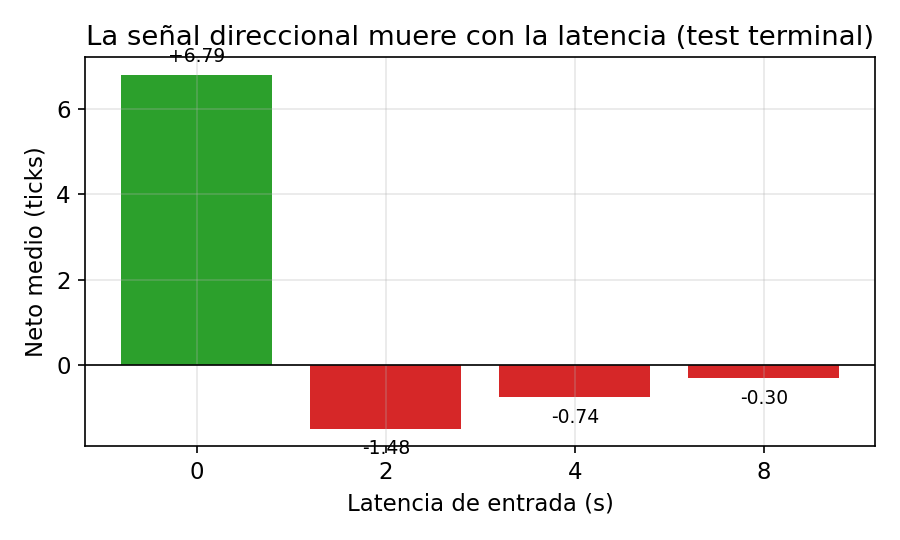
\includegraphics[width=0.7\textwidth]{figures/fig_latencia.png}
\caption{Neto medio en el test terminal frente a la latencia de entrada. La señal a latencia
nula es real como \emph{markout} desde el instante de la señal, pero no sobrevive como
política ejecutable con dos segundos de latencia.}
\label{fig:latencia}
\end{figure}

Este es el resultado que vertebra todo el trabajo: \textbf{acertar la dirección no equivale
a obtener beneficio}. Con una latencia realista de dos segundos, el neto medio del test
terminal cae a $-1{,}48$ ticks. El problema deja de ser de clasificación y pasa a ser de
ejecución; a partir de aquí, todo modelo se evalúa por su política económica bajo coste y
latencia, no por su acierto.

\section{Metodología y entrenamiento}

\subsection{Definición del objetivo}

Para cada instante $t$ se define el retorno futuro del precio medio a un horizonte $H$,
\begin{equation}
\Delta_H(t) = \frac{m_{t+H} - m_t}{m_t},
\end{equation}
donde $m_t$ es el precio medio del contrato. La etiqueta direccional se obtiene con un
umbral $\theta$ que absorbe el \emph{spread}, las comisiones y el ruido:
\begin{equation}
y_t = \begin{cases}
\textsc{up} & \text{si } \Delta_H(t) > \theta,\\[2pt]
\textsc{down} & \text{si } \Delta_H(t) < -\theta,\\[2pt]
\textsc{flat} & \text{en otro caso.}
\end{cases}
\end{equation}
Esta etiqueta ternaria es útil para mirar el arco experimental en su conjunto; el
especialista final, en cambio, usa los dos objetivos económicos que se definen más abajo.
Las características son causales (solo usan información hasta
$t$) y las etiquetas se calculan \emph{a posteriori} de forma trazable, de modo que no
entra información del futuro por las entradas del modelo. Todos los resultados económicos se
expresan en ticks netos, que es la unidad natural del libro; no se traducen a dinero porque
ello exigiría suponer un tamaño de posición y favorecería la sobreafirmación.

\paragraph{Los dos objetivos del especialista.} El modelo final no usa la etiqueta ternaria,
sino dos objetivos complementarios, porque un modelo que debe decidir si entra necesita
saber algo más fino que la dirección: cuánto vale la operación y si el entorno de ejecución
es favorable (Figura~\ref{fig:doscabezas}).

\begin{figure}[h]
\centering
\begin{tikzpicture}[
  node distance=5mm and 12mm, font=\small, >=Latex,
  io/.style={draw, rounded corners, fill=blue!6, align=center, minimum width=30mm, minimum height=9mm},
  head/.style={draw, rounded corners, fill=orange!12, thick, align=center, minimum width=42mm, minimum height=11mm},
  dec/.style={draw, rounded corners, fill=green!10, align=center, minimum width=34mm, minimum height=11mm},
]
\node[io] (x) {36 características\\causales (\emph{no\_clock})};
\node[head, right=of x, yshift=9mm] (reg) {Regresor EV\\\texttt{exec\_net\_cost\_0p25}};
\node[head, right=of x, yshift=-11mm] (clf) {Clasificador salud\\\texttt{healthy\_fill\_proxy}};
\node[dec, right=14mm of $(reg)!0.5!(clf)$] (pol) {Operar si\\EV $>0{,}75$ \emph{y}\\P(salud)$\ge 0{,}50$};
\draw[-{Latex}] (x.east) -- (reg.west);
\draw[-{Latex}] (x.east) -- (clf.west);
\draw[-{Latex}] (reg.east) -- (pol.west);
\draw[-{Latex}] (clf.east) -- (pol.west);
\end{tikzpicture}
\caption{Modelo de dos cabezas. Un regresor predice el valor esperado de la operación y un
clasificador predice si el relleno será ``sano''. La política exige ambas condiciones.}
\label{fig:doscabezas}
\end{figure}

El \textbf{regresor} predice \texttt{exec\_net\_cost\_0p25\_H60}: el neto ejecutado a 60
segundos tras descontar una fracción (0,25) del coste visible de entrada de cada operación.
El \textbf{clasificador} predice \texttt{healthy\_fill\_proxy\_0p25\_H60}: una variable
binaria que vale 1 cuando ese neto es positivo \emph{y} la operación no cae en el peor
cuartil de un grupo de operaciones comparables (mismo bloque temporal, fase, nivel de
\emph{spread}, microprice y momento del perp). La independencia entre ambas cabezas es
deliberada: una operación puede tener alto valor esperado pero baja probabilidad de relleno
sano si el libro está degradado.

\subsection{Validación temporal y prevención de fuga}

La partición respeta siempre el orden del tiempo: el entrenamiento utiliza las sesiones más
antiguas, la validación las posteriores y el test terminal el bloque final. En los
experimentos secuenciales se emplea además un protocolo fuera de pliegue
(\emph{out-of-fold}): cada modelo se entrena solo con días anteriores, las predicciones que
consume una segunda etapa son siempre fuera de muestra, y la política de decisión se
selecciona sin observar el test terminal. Esta disciplina contra la fuga temporal es la
salvaguarda frente a resultados ilusorios~\cite{lopezdeprado2018,gu2020empirical}.

\subsection{Modelo de costes y latencia}

La latencia no se supone, se mide. En una prueba controlada del ciclo de orden de
Polymarket, el tiempo entre observar la oportunidad y confirmar el emparejamiento fue de
unos 0,43 segundos en el percentil 95 de la muestra válida. Aun así, por prudencia se
trabaja con cifras peores: una latencia conceptual de un segundo y una latencia observable
en los datos de dos segundos (la malla de captura). El coste de ejecución no se fija como un
número plano de ticks, sino como una fracción del coste visible de entrada de cada
operación: la mitad de ese coste como referencia, un cuarto como contraste optimista y el
coste completo como prueba de estrés. Modelar el coste relativo al libro de cada instante es
más fiel que asumir un coste fijo e igual para todas las operaciones. Formalmente, el neto
ejecutado a horizonte $H$ con un factor de coste $c \in \{0,\ 0{,}25,\ 0{,}5,\ 1\}$ es
\begin{equation}
\text{net}_c(t) = \big(\Delta^{\text{ticks}}_H(t) - b\big) - c \cdot \kappa_t,
\label{eq:coste}
\end{equation}
donde $\Delta^{\text{ticks}}_H(t)$ es el \emph{markout} en ticks desde la entrada (a dos
segundos del instante de señal) hasta el horizonte, $b$ es un \emph{buffer} fijo y $\kappa_t$
es el coste visible de entrada de esa operación. Nótese que, por construcción, un factor de
coste mayor produce un neto menor sobre la misma operación; por eso el resultado al coste de
referencia ($c=0{,}5$) es siempre inferior al optimista ($c=0{,}25$) y superior al de estrés
($c=1$).

\subsection{Métricas de evaluación}

La elección de métricas es deliberada y responde a las características del problema. Para la
fase de clasificación no se reporta la precisión bruta (\emph{accuracy}), porque el dominio
de la clase \textsc{flat} la vuelve engañosa; en su lugar se usan la \textbf{precisión
equilibrada} (\emph{balanced accuracy}) y la \textbf{F1 macro}, que promedian por clase y no
premian al modelo que siempre predice quietud. Para medir la capacidad de \emph{ordenar} las
oportunidades se emplea el \textbf{AUC} (área bajo la curva ROC), independiente del umbral.

Ahora bien, la métrica que decide es económica, no de clasificación: el \textbf{neto medio
por operación} bajo el modelo de costes de la ecuación~\eqref{eq:coste}. A su alrededor se
reportan siempre cuatro elementos de soporte e incertidumbre: (i) el \textbf{número de
operaciones y de días}, porque un neto sin soporte no es interpretable; (ii) un
\textbf{intervalo de confianza \emph{bootstrap}} (5\,000 remuestreos, semilla fija); (iii) la
\textbf{probabilidad de neto positivo} estimada sobre esa misma distribución; y (iv) el
\textbf{drawdown máximo} y el número de \textbf{días positivos}, como medidas de estabilidad.
Esta batería evita confundir una señal estadística con una estrategia viable.

\subsection{La escalera de modelos}

Los modelos se evalúan en una progresión incremental, de menor a mayor complejidad,
exigiendo en cada salto que la complejidad añadida se justifique con evidencia de mejora
bajo el mismo protocolo de costes y validación (Figura~\ref{fig:escalera}).

\begin{figure}[h]
\centering
\begin{tikzpicture}[
  node distance=4mm, font=\small, >=Latex,
  rung/.style={draw, rounded corners, align=center, minimum width=0.84\textwidth, minimum height=8mm, inner sep=3pt},
]
\node[rung, fill=blue!6] (s1) {Línea base tabular H16 (acierto $\sim$90\,\%, pero muere con latencia)};
\node[rung, fill=blue!6, below=of s1] (s2) {Modelos sensibles a la latencia (AUC 0,79; política negativa)};
\node[rung, fill=blue!8, below=of s2] (s3) {Secuencias y libro: GRU, Conv1D (\emph{BookEncoder}), fusión, TCN (representación sí, política no)};
\node[rung, fill=orange!10, below=of s3] (s4) {Corrección del \emph{score} de selección adversa; selección de horizonte (H60)};
\node[rung, fill=green!12, thick, below=of s4] (s5) {Especialista \emph{prestart} H60 (HGB de dos cabezas) + filtro de volatilidad};
\draw[-{Latex}] (s1)--(s2); \draw[-{Latex}] (s2)--(s3); \draw[-{Latex}] (s3)--(s4); \draw[-{Latex}] (s4)--(s5);
\end{tikzpicture}
\caption{La escalera de modelos. Cada paso debe superar al anterior bajo el mismo protocolo;
si no lo hace, se descarta.}
\label{fig:escalera}
\end{figure}

Los \textbf{modelos sensibles a la latencia} incorporan la latencia en el etiquetado y la
selección; uno de ellos alcanza un AUC de test de 0,79 y, pese a ello, su política económica
sigue siendo negativa. Sobre el \textbf{libro de órdenes} se construyen secuencias de ocho
pasos y un tensor de los diez primeros niveles, y se evalúan una red recurrente (GRU, capa
oculta de dimensión 56), un codificador convolucional del libro (\emph{BookEncoder}, dos
capas Conv1D con \emph{pooling} medio y máximo, inspirado en
DeepLOB~\cite{zhang2019deeplob,tsantekidis2017}), una fusión de ambos y una red convolucional
temporal (TCN) para el régimen de volatilidad. El \emph{BookEncoder} resume cada fotografía
del libro con dos convoluciones unidimensionales sobre la dimensión de niveles y un
\emph{pooling} dual (medio y máximo):
\begin{equation}
\mathbf{h} = \big[\operatorname{mean}_\tau\, \phi(\mathbf{B}_\tau)\ \|\ \operatorname{max}_\tau\, \phi(\mathbf{B}_\tau)\big],
\quad
\phi = \text{ReLU}\!\circ\!\text{Conv1d}\!\circ\!\text{Dropout}\!\circ\!\text{ReLU}\!\circ\!\text{Conv1d},
\end{equation}
donde $\mathbf{B}_\tau$ es el libro en el paso $\tau$ de la secuencia y $\|$ denota
concatenación. El \emph{pooling} máximo capta los picos de profundidad, a menudo más
informativos que la media en mercados poco líquidos. Estas arquitecturas aprenden
representación, pero no producen una política estable con un horizonte de entrenamiento de
unas dos semanas (unos 5\,800 ejemplos): el aprendizaje profundo se aparca a la espera de
más datos.

Durante la auditoría se detectó y corrigió un error de interpretación en el \emph{score} de
selección adversa (su orientación correcta es $1 - P(\text{adverso})$), lo que ilustra que
una métrica positiva no basta sin auditar su significado económico. Por último, al comparar
horizontes (Tabla~\ref{tab:horizonte}), solo H60 conserva señal; H120 y H240 colapsan, por
lo que H60 queda como único candidato.

\begin{table}[h]
\centering
\caption{Selección de horizonte (ticks netos \emph{proxy}). Solo H60 conserva señal.}
\label{tab:horizonte}
\begin{tabular}{lrr}
\toprule
\textbf{Métrica} & \textbf{H60} & \textbf{H120} \\
\midrule
AUC test                       & $0{,}565$ & $0{,}495$ \\
Top 35\,\% test, coste $0{,}5$ & $+0{,}426$ & $-1{,}117$ \\
Top 35\,\% test, coste $1{,}0$ & $+0{,}058$ & $-1{,}491$ \\
\bottomrule
\end{tabular}
\end{table}

\subsection{Especialista \emph{prestart} H60}

El candidato final es un especialista para la ventana \emph{prestart}: un modelo de
\emph{gradient boosting} sobre histogramas (HistGradientBoosting) con las dos cabezas
descritas, entrenado sobre 36 características sin variables de reloj (para evitar atajos
temporales triviales). La señal se restringe a la ventana de $-60$ a $-45$ segundos respecto
a la apertura, con libro saludable y coste visible acotado (Figura~\ref{fig:prestart}).

\begin{figure}[h]
\centering
\begin{tikzpicture}[font=\small, >=Latex]
  \draw[-{Latex}] (-0.5,0) -- (10.8,0) node[right, font=\scriptsize] {tiempo};
  \fill[orange!25] (1,-0.18) rectangle (3.5,0.18);
  \node[font=\scriptsize, align=center] at (2.25,0.6) {ventana \emph{prestart}\\$-60$ a $-45$\,s};
  \draw[dashed] (8.5,-0.7) -- (8.5,0.9);
  \node[font=\scriptsize, align=center] at (8.5,1.1) {apertura\\del mercado};
  \foreach \x/\lab in {1/{$-60$\,s}, 3.5/{$-45$\,s}, 8.5/{$0$}}
    \draw (\x,0.12) -- (\x,-0.12) node[below, font=\scriptsize] {\lab};
  \node[font=\scriptsize, align=center, gray] at (5.9,-0.6) {(resto del \emph{prestart}: no se opera)};
\end{tikzpicture}
\caption{La ventana \emph{prestart} del especialista: solo se opera entre $-60$ y $-45$
segundos respecto a la apertura del mercado, donde el análisis exploratorio detectó una
densidad atípica de actividad del libro.}
\label{fig:prestart}
\end{figure} Ambas cabezas comparten una
configuración de regularización agresiva (tasa de aprendizaje 0,045, hasta 220 iteraciones
con parada anticipada, máximo de 15 hojas por árbol, mínimo de 120 muestras por hoja y
regularización L2 de 0,10), necesaria porque el bloque de entrenamiento del especialista
tiene del orden de mil observaciones útiles. La política congelada opera cuando el valor
esperado predicho supera 0,75 y la probabilidad de salud no baja de 0,50; ambos umbrales se
seleccionaron sobre el conjunto de validación, nunca sobre el test terminal.

\subsection{Filtro de volatilidad}

Al preparar la validación fuera de muestra se observó un cambio de régimen: la fracción de
sesiones de alta volatilidad pasó de un 18--22\,\% en entrenamiento a alrededor del 58\,\% en
el conjunto fuera de muestra (véase la Figura~\ref{fig:regimen} del
Capítulo~\ref{ch::resultados}). Como el modelo aprendió en un régimen de baja volatilidad y
sus predicciones en alta volatilidad no son fiables bajo la distribución desplazada, se
introduce un filtro simple que solo habilita la operativa cuando la volatilidad realizada a
cinco segundos no supera el umbral 0,6657, correspondiente al percentil 80 de la volatilidad
de entrenamiento (un umbral fijado con los datos antiguos, no ajustado a los nuevos).

\subsection{Protocolo de congelación}
\label{sec:congelacion}

El candidato final —modelo, conjunto de características y umbrales de política— se congeló
antes de observar el conjunto fuera de muestra del 6 al 10 de junio. Esta decisión convierte
la validación posterior en una prueba fuera de muestra genuina, y previene el sobreajuste por
selección múltiple~\cite{bailey2014deflated}. Una vez fijada, la política no se reajusta para
mejorar los resultados.

% called by main.tex
%
\chapter{Resultados y análisis}
\label{ch::resultados}

Este capítulo separa dos niveles de evidencia que no deben confundirse. Primero se presenta
la evaluación confirmatoria del especialista base, congelado antes de observar el bloque del
6 al 10 de junio. Después se documenta el diagnóstico de volatilidad realizado sobre ese mismo
bloque. El segundo resultado es útil para formular una política futura, pero no constituye
una nueva validación fuera de muestra.

\section{Resultados obtenidos}

\subsection{Validación fuera de muestra del especialista base}

El especialista congelado selecciona 754 unidades de acción en los cinco días fuera de
muestra. Sin aplicar ningún filtro decidido a partir de esos datos, obtiene un neto medio de
$+0{,}349$ ticks al coste de referencia. El promedio es positivo en tres de cinco días y
pasa a ser ligeramente negativo ($-0{,}026$ ticks) cuando se carga el coste visible completo
(Tabla~\ref{tab:fresh}). Esta es la estimación limpia del rendimiento fuera de muestra.

\begin{table}[h]
\centering
\caption{Validación fuera de muestra del especialista base congelado. Los valores son ticks
netos por unidad de acción y no incorporan el filtro de volatilidad posterior.}
\label{tab:fresh}
\begin{tabular}{lr}
\toprule
\textbf{Métrica} & \textbf{Valor} \\
\midrule
Unidades de acción ($n$)                  & 754 \\
Días de soporte                          & 5 (3/5 positivos) \\
Neto medio (coste 0,25, optimista)         & $+0{,}537$ ticks \\
Neto medio (coste 0,5, referencia)         & $+0{,}349$ ticks \\
Neto medio (coste 1,0, estrés)             & $-0{,}026$ ticks \\
\bottomrule
\end{tabular}
\end{table}

\begin{table}[h]
\centering
\caption{Desglose diario del especialista base al coste de referencia.}
\label{tab:base_daily}
\begin{tabular}{lrr}
\toprule
\textbf{Día} & \textbf{$n$} & \textbf{Neto medio @0,5} \\
\midrule
6 de junio  & 220 & $+0{,}666$ \\
7 de junio  &  97 & $+1{,}342$ \\
8 de junio  & 241 & $+0{,}308$ \\
9 de junio  & 146 & $-0{,}565$ \\
10 de junio &  50 & $-0{,}105$ \\
\bottomrule
\end{tabular}
\end{table}

El signo positivo al coste de referencia indica que el especialista conserva una señal
modesta donde los modelos anteriores habían fracasado. Sin embargo, ni la estabilidad diaria
ni el escenario de coste completo permiten calificarlo como una política robusta. La lectura
defendible es, por tanto, \emph{señal parcial fuera de muestra}, no rentabilidad demostrada.

\subsection{Diagnóstico \emph{post-hoc} del régimen de volatilidad}

La inspección del bloque reveló que la fracción de sesiones de alta volatilidad aumentó hasta
aproximadamente el 58\,\%, frente al 18--22\,\% de los periodos históricos
(Figura~\ref{fig:regimen}). Para estudiar ese desplazamiento se dividió la selección con el
umbral 0,6657, percentil 80 de la volatilidad de entrenamiento. El umbral numérico no se
ajustó al bloque nuevo, pero la decisión de usarlo como filtro sí se tomó tras observarlo; por
ello, todo lo que sigue en esta subsección es diagnóstico y exploratorio.

\begin{figure}[h]
\centering
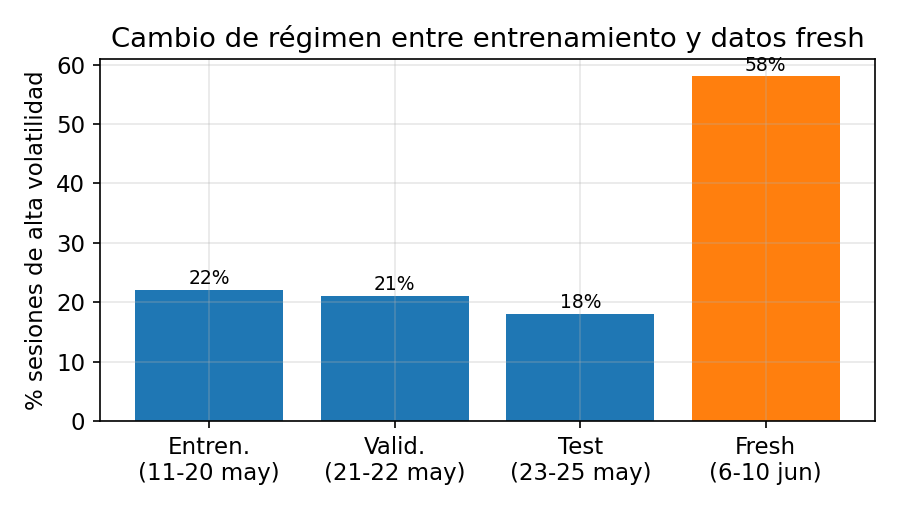
\includegraphics[width=0.6\textwidth]{figures/fig_regimen.png}
\caption{Fracción de sesiones de alta volatilidad por periodo. El salto del bloque nuevo
motiva el análisis de régimen, pero no valida por sí mismo el filtro.}
\label{fig:regimen}
\end{figure}

La Tabla~\ref{tab:regimen} muestra el contraste. Hay 318 acciones de baja volatilidad, 435 de
alta volatilidad y una acción sin dato de volatilidad, que una regla operativa conservadora
rechazaría. Las primeras son positivas y las segundas, negativas al coste de referencia.

\begin{table}[h]
\centering
\caption{Diagnóstico \emph{post-hoc} por régimen en el bloque del 6--10 de junio (ticks por
unidad de acción).}
\label{tab:regimen}
\begin{tabular}{lrrrr}
\toprule
\textbf{Régimen} & \textbf{$n$} & \textbf{@0,25} & \textbf{@0,5} & \textbf{@1,0} \\
\midrule
Baja volatilidad   & 318 & $+1{,}258$ & $+1{,}069$ & $+0{,}691$ \\
Alta volatilidad   & 435 & $+0{,}004$ & $-0{,}183$ & $-0{,}558$ \\
Volatilidad ausente&   1 & $+3{,}327$ & $+3{,}154$ & $+2{,}807$ \\
\midrule
Total sin filtro   & 754 & $+0{,}537$ & $+0{,}349$ & $-0{,}026$ \\
\bottomrule
\end{tabular}
\end{table}

\begin{figure}[h]
\centering
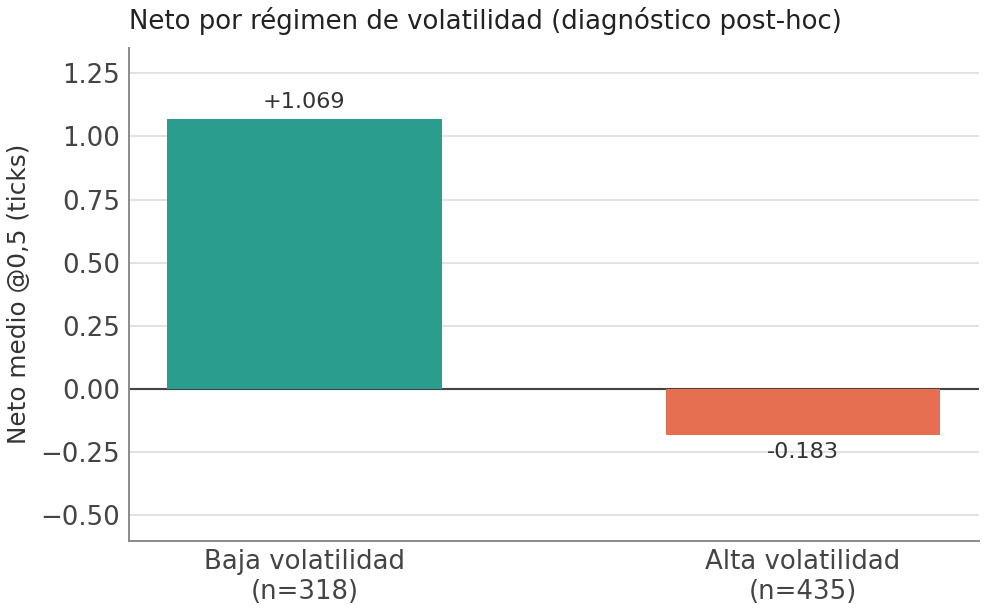
\includegraphics[width=0.56\textwidth]{figures/fig_regimen_neto.png}
\caption{Contraste \emph{post-hoc} del neto medio entre baja y alta volatilidad. La separación
es una hipótesis de política que requiere datos posteriores.}
\label{fig:regimenneto}
\end{figure}

Si se aplica retrospectivamente el filtro de baja volatilidad, el subconjunto de 318 acciones
mantiene signo positivo en los tres niveles de coste (Figura~\ref{fig:coste}) y en los cinco
días (Figura~\ref{fig:netodiario}). Su suma cronológica presenta un drawdown diagnóstico de
88,1 ticks (Figura~\ref{fig:drawdown}). Estas magnitudes describen el subconjunto observado;
no son PnL de una cartera ejecutada.

\begin{figure}[h]
\centering
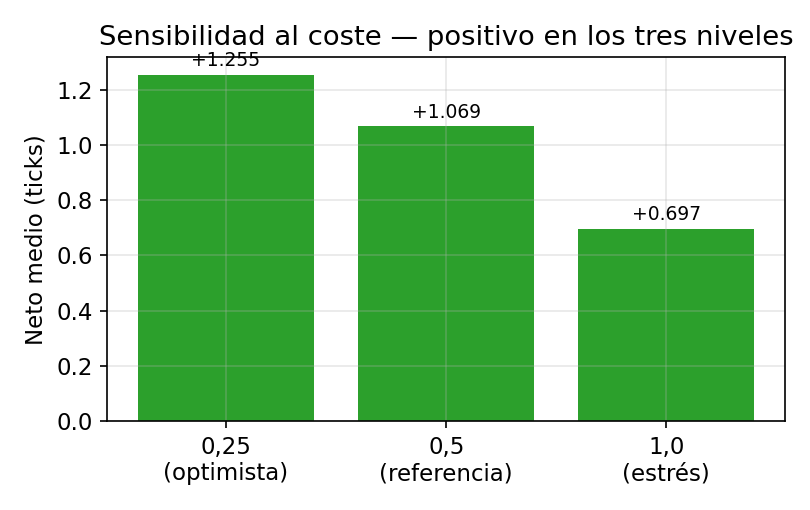
\includegraphics[width=0.55\textwidth]{figures/fig_coste.png}
\caption{Sensibilidad al coste del subconjunto de baja volatilidad. Resultado exploratorio
obtenido tras inspeccionar el mismo bloque.}
\label{fig:coste}
\end{figure}

\begin{figure}[h]
\centering
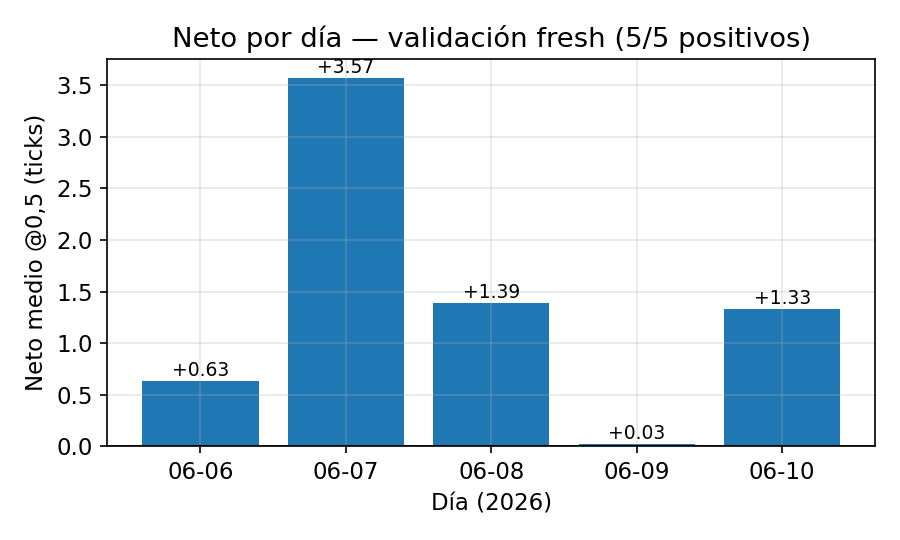
\includegraphics[width=0.62\textwidth]{figures/fig_neto_diario.png}
\caption{Neto medio diario del subconjunto \emph{post-hoc} de baja volatilidad.}
\label{fig:netodiario}
\end{figure}

\begin{figure}[h]
\centering
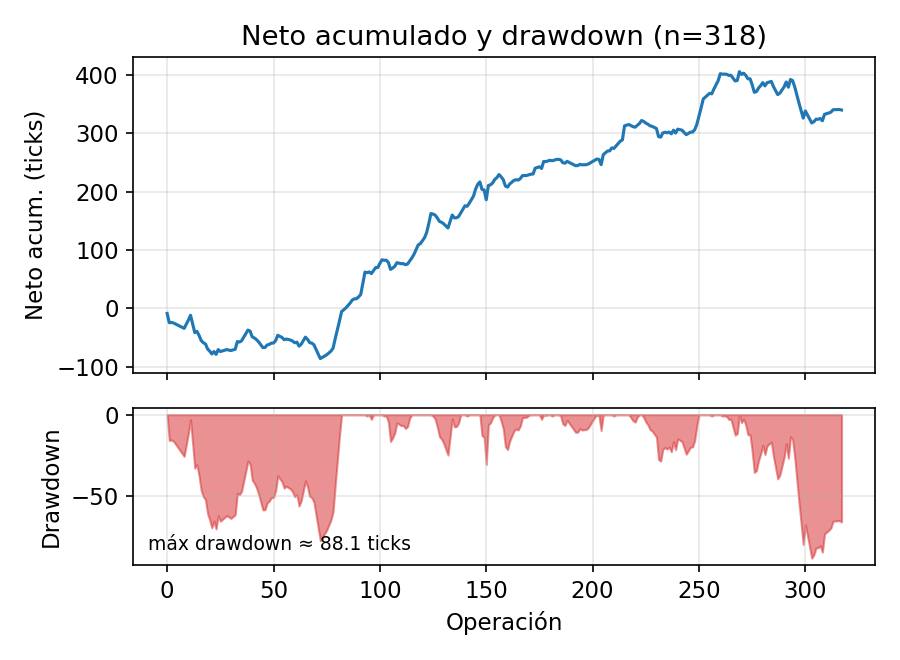
\includegraphics[width=0.62\textwidth]{figures/fig_drawdown.png}
\caption{Suma acumulada y drawdown diagnóstico de 318 unidades de acción. No representa una
cartera con restricciones de capital o de exposición simultánea.}
\label{fig:drawdown}
\end{figure}

El remuestreo independiente de las 318 acciones produce un IC90 de
$[+0{,}472,+1{,}654]$ y $P=0{,}998$, pero esa estimación ignora la dependencia entre señales
del mismo mercado. Hay 156 mercados y hasta ocho acciones por mercado. Un \emph{bootstrap}
agrupado por mercado amplía el IC90 a $[+0{,}193,+2{,}004]$ y reduce la probabilidad estimada
a 97,6~\%. Ambos cálculos son descriptivos: la selección \emph{post-hoc} impide darles una
lectura confirmatoria.

\subsection{Registro de sombra retrospectivo}

Para auditar la mecánica de la política candidata se construyó un registro de sombra
\emph{offline}: conserva cada unidad de acción, su mercado, el resumen diario y las reglas de
promoción. Es una reproducción retrospectiva de lo que la regla habría indicado, no una
ejecución prospectiva ni un sistema activo en tiempo real. El filtro queda congelado después
del 10 de junio; solo observaciones posteriores pueden contar para las puertas de promoción.

Además, varias señales pertenecen al mismo mercado y sus horizontes H60 se solapan. Por ello
se denominan \emph{unidades de acción}, no operaciones independientes, y la suma acumulada no
incorpora una regla de exposición máxima. Una futura sombra prospectiva deberá decidir si
permite apilar posiciones o admite una sola posición por mercado.

\section{Comparativa con otros enfoques y baseline}

Esta sección sitúa el resultado limpio del especialista frente a las alternativas evaluadas:
las arquitecturas profundas sobre el libro de órdenes y los intentos de adaptación al cambio
de régimen. La comparación justifica por qué la mejor señal disponible procede de un modelo
tabular sencillo y no de una red profunda.

\subsection{Especialista tabular frente a aprendizaje profundo}

Las redes recurrentes y convolucionales sobre el libro aprenden representación ---algunas
políticas \emph{proxy} resultan positivas dentro de muestra---, pero esa ventaja no sobrevive
cuando se exige selección causal día a día y estabilidad en todo el bloque de test. Con unas
dos semanas de datos, la capacidad necesaria para generalizar temporalmente excede lo que
las redes pueden estimar de forma fiable.

El modelo tabular con regularización agresiva opera en el extremo opuesto: aumenta su sesgo
pero reduce drásticamente la varianza. Restringir la señal a la ventana \emph{prestart} acota
el espacio de hipótesis. Esa combinación conserva un promedio positivo al coste de referencia
en el bloque intacto, aunque todavía no supera el coste de estrés. El resultado no descarta el
aprendizaje profundo; lo sitúa como una vía a reevaluar cuando el volumen de datos crezca.

\subsection{Experimentos de adaptación al régimen}

Ante el cambio de régimen se probaron reentrenamiento incremental con ventana móvil,
alineación de correlaciones CORAL~\cite{sun2016coral}, un filtro conformal, un
\emph{ensemble} por \emph{bootstrap}, un filtro de volatilidad adaptativo, características
normalizadas por volatilidad y \emph{distillation} de una red convolucional temporal.
Ninguna alternativa produjo evidencia prospectiva robusta con tan pocos días. Este resultado
negativo sigue siendo informativo, pero no permite declarar vencedor al filtro simple sobre
el mismo bloque usado para proponerlo. La comparación definitiva queda aplazada hasta disponer
de nuevos datos bajo una política ya congelada.

% called by main.tex
%
\chapter{Despliegue}
\label{ch::despliegue}

Este capítulo, opcional en la plantilla, documenta la \emph{estrategia} de despliegue. La
decisión más importante es deliberada y se explica a continuación: el sistema \textbf{no se
despliega} con capital real, sino que se detiene en una fase de seguimiento en sombra
(\emph{paper-shadow}).

\section{Estrategia de despliegue y seguimiento en paper-shadow}

Esta sección justifica la decisión de no desplegar el sistema en producción, describe la
infraestructura de seguimiento en sombra que se utiliza en su lugar y esboza qué requeriría
un despliegue futuro. La decisión de detenerse es coherente con la prudencia metodológica que
guía todo el trabajo.

\subsection{Por qué no se despliega}

Desplegar una política de decisión económica con cinco días de soporte fuera de muestra
sería metodológicamente imprudente, por mucho que el intervalo de confianza sea estrecho y
los cinco días positivos. Cinco días no constituyen una validación definitiva, y un sistema
que opera con capital real es especialmente sensible al sobreajuste cuando el horizonte de
datos es reducido. Por coherencia con la tesis del trabajo —que la honestidad del protocolo
prevalece sobre cualquier número concreto— el proyecto se detiene antes de operar.

\subsection{Seguimiento \emph{paper-shadow}}

En su lugar, el sistema se mantiene en \emph{paper-shadow}: se registra, operación a
operación, lo que la política \emph{habría} hecho, sin arriesgar capital. Esta
infraestructura produce una contabilidad detallada, un resumen diario y, sobre todo, una
puerta de decisión cuantitativa que determina cuándo —si alguna vez— tendría sentido pasar a
una fase superior. Las reglas de promoción son deliberadamente conservadoras y exigen
soporte temporal, no solo neto positivo:

\begin{itemize}[noitemsep]
  \item \textbf{Candidato a paper-shadow:} neto superior a 0,5 ticks, al menos 200
  operaciones y al menos 8 días de soporte.
  \item \textbf{Candidato a despliegue:} neto superior a 0,5 ticks, al menos 400 operaciones
  y al menos 12 días de soporte.
\end{itemize}

Con los datos actuales (318 operaciones, 5 días), el candidato no alcanza el primer umbral
por falta de días, y queda explícitamente en estado \emph{prometedor pero con datos
insuficientes}.

\subsection{Diseño de una hipotética API de inferencia}

A título de trabajo futuro, y solo si se superasen las puertas de promoción anteriores, un
despliegue eventual tomaría la forma de un servicio de inferencia con cuatro etapas
encadenadas. Primero, una etapa de ingesta que reconstruyese en tiempo real el estado del
mercado sobre la malla de dos segundos a partir de las mismas fuentes de captura. Segundo,
una etapa de cálculo que generase las 36 características causales del instante actual,
idéntica a la del entrenamiento para evitar discrepancias entre entrenamiento y producción
(\emph{train/serve skew}). Tercero, una etapa de decisión que consultase las dos cabezas del
especialista y devolviese una recomendación (operar o no) junto con el valor esperado y la
probabilidad de salud. Y cuarto, una capa de guardas que aplicase, antes de cualquier
recomendación, los filtros estrictos de entorno, el filtro de volatilidad y un mecanismo de
inhibición que cortase la operativa ante datos obsoletos o degradados.

Por encima de ese servicio operaría una capa de monitorización que vigilase la deriva de
distribución (especialmente el régimen de volatilidad), registrase cada decisión para
auditoría y dispusiese de un interruptor de parada inmediata. Conviene insistir en que esta
arquitectura es un \emph{diseño}, no una implementación: su desarrollo solo tendría sentido
tras acumular el soporte temporal que hoy falta, y siempre manteniendo el principio de
detenerse ante cualquier señal de degradación.

% called by main.tex
%
\chapter{Aspectos éticos y limitaciones}
\label{ch::etica}

Este capítulo recoge las consideraciones éticas que han guiado el trabajo y una revisión
explícita de sus limitaciones, que delimitan el alcance de cualquier conclusión.

\section{Consideraciones éticas}

El sistema estudia decisiones económicas automatizadas y es especialmente sensible al
sobreajuste cuando el horizonte de datos es reducido. La actuación responsable es no operar
con capital real y no convertir un diagnóstico \emph{post-hoc} en una afirmación de
rentabilidad. La política completa queda congelada para observación prospectiva, sin que los
días usados para formularla cuenten de nuevo como validación.

En cuanto a los datos, se adopta un marco de confidencialidad, integridad y disponibilidad.
Una referencia externa retrasada o errónea puede inducir una señal espuria; por ello el
sistema se entrena solo con sesiones aceptadas, separa datos crudos, características y
etiquetas, mantiene trazabilidad de los artefactos e inhibe la operativa ante datos
obsoletos. El trabajo emplea datos públicos de mercado y no datos personales. El corpus
completo no se distribuye por tamaño; se publican el esquema, un ledger anonimizado de
acciones y el código de evaluación.

\section{Limitaciones}

\textbf{Selección posterior al bloque.} El especialista base sí estaba congelado y su
resultado limpio es $+0{,}349$ ticks por acción al coste de referencia. El filtro de
volatilidad se incorporó después de observar el cambio de régimen; por tanto, su resultado de
$+1{,}069$ ticks sobre el mismo bloque es exploratorio y necesita fechas posteriores.

\textbf{Soporte temporal.} El conjunto fuera de muestra abarca cinco días. Tres de cinco son
positivos para la política base y cinco de cinco dentro del subconjunto diagnóstico. Ninguna
de las dos cifras constituye una validación definitiva.

\textbf{Dependencia y solapamiento.} Las 318 unidades del diagnóstico pertenecen a 156
mercados, con hasta ocho señales por mercado y horizontes H60 solapados. El
\emph{bootstrap} por filas subestima esa dependencia. Un remuestreo agrupado por mercado
amplía el IC90\,\% a $[+0{,}193,+2{,}004]$, pero sigue describiendo un subconjunto elegido
\emph{post-hoc}. Además, no se ha fijado una regla de exposición simultánea; por ello la suma
acumulada no es PnL de cartera.

\textbf{Validación \emph{offline}.} La evaluación usa un modelo de ejecución conservador pero
simplificado. No reconstruye la cola orden por orden ni incorpora rellenos parciales. El
registro de sombra actual es retrospectivo; falta una ejecución prospectiva de mayor
fidelidad.

\textbf{Reproducibilidad parcial.} El repositorio permite recalcular las tablas públicas desde
el ledger anonimizado y probar la lógica compartida. La reproducción integral del
entrenamiento requiere el corpus privado de gran tamaño y se documenta como limitación, no
como capacidad publicada.

\textbf{Patrón en U.} Dentro de la baja volatilidad se observa una posible relación en forma de
U entre volatilidad y resultado. Como se descubrió en los mismos cinco días, se conserva solo
como hipótesis para trabajo futuro.

% called by main.tex
%
\chapter{Reproducibilidad}
\label{ch::reproducibilidad}

\section{Enlace a repositorio GitHub}

El código, los registros de resultados y los artefactos públicos de auditoría se mantienen en
un repositorio:

\begin{center}
\url{https://github.com/marcmaldonadolorca/polymarket-btc-microstructure}
\end{center}

\subsection{Estructura del repositorio}

El repositorio se organiza en los siguientes directorios:

\begin{description}[align=right,labelwidth=2.6cm]
\item [\texttt{config/}] Umbrales congelados de la política y configuraciones del arco.
\item [\texttt{docs/}] Documentos canónicos del proceso, renumerados de forma secuencial.
\item [\texttt{notebooks/}] Cuadernos pedagógicos ejecutados (EDA, particiones, objetivo,
línea base, latencia, secuencias, corrección del \emph{score} adverso y especialista).
\item [\texttt{scripts/}] Puntos de entrada reproducibles de cada experimento.
\item [\texttt{src/}] Paquete con la lógica compartida (datos, características, modelos,
evaluación), con pruebas automatizadas.
\item [\texttt{results/}] Tablas de resultados y ledger anonimizado de 754 unidades de acción.
\item [\texttt{sql/}] Esquema de la consulta base de entrenamiento.
\item [\texttt{reports/}] Esta memoria (fuente LaTeX).
\end{description}

\subsection{Cómo reproducir}

El entorno se prepara con un entorno virtual de Python y la instalación de las dependencias
declaradas. Las pruebas automatizadas verifican la lógica de política y sus guardas. El ledger
\texttt{results/final\_candidate\_actions\_anonymized.csv} permite recalcular las tablas
agregadas, los desgloses por régimen y la incertidumbre agrupada sin acceder al corpus
completo. El script que lo genera queda versionado para mantener trazabilidad, aunque su
ejecución integral requiere el workspace privado de investigación.

\subsection{Datos no publicados}

El conjunto completo (del orden de 2,6 millones de filas \emph{cross-venue}, más la base de
captura) no se publica por tamaño. En su lugar se incluyen el esquema SQL, un ledger
anonimizado suficiente para reproducir las cifras finales y el código del \emph{pipeline}.
Esto permite una auditoría parcial, no la reproducción bit a bit del entrenamiento. Declarar
esa frontera de forma explícita es parte de la trazabilidad y reduce la deuda técnica propia de
estos sistemas~\cite{sculley2015debt}.

% called by main.tex
%
\chapter{Conclusiones}
\label{ch::conclusiones}

Este trabajo ha presentado una metodología de captura de datos, validación temporal y control
de costes para la predicción de corto plazo en mercados de Bitcoin de Polymarket. La
conclusión central es que una precisión direccional cercana al 90\,\% no garantiza una política
económica: con una latencia de entrada realista, el coste y la ejecución dominan el resultado.

El aprendizaje profundo aplicado a secuencias y al libro de órdenes aprende representaciones
útiles, pero no produce una política estable con unas dos semanas de datos. El especialista
tabular congelado conserva una señal modesta en cinco días intactos fuera de muestra:
$+0{,}349$ ticks por unidad al coste de referencia, 754 unidades y tres de cinco días
positivos; bajo el coste completo, el promedio es $-0{,}026$ ticks.

El análisis posterior detecta un cambio de régimen y propone un filtro de baja volatilidad.
Sobre el mismo bloque, ese subconjunto alcanza $+1{,}069$ ticks y cinco de cinco días
positivos. Su valor es el de una hipótesis prometedora, no el de una validación confirmatoria:
la regla se congela después del diagnóstico y queda pendiente de datos futuros.

Las aportaciones del trabajo son cuatro: un sistema de captura y control de calidad
multifuente; un protocolo temporal que incorpora coste y latencia medidos; evidencia
cuantitativa de la ruptura entre predicción y ejecución; y una trazabilidad que conserva tanto
los resultados negativos como la corrección de errores metodológicos. No se afirma
rentabilidad real ni se presenta un bot listo para desplegar.

\paragraph{Trabajo futuro.} La prioridad es ejecutar prospectivamente la política completa
sin retocar umbrales, con una sola regla de exposición por mercado y registro de fills. Solo
después podrá evaluarse el filtro de volatilidad. Con un horizonte de datos sustancialmente
mayor podrán reevaluarse arquitecturas como el \emph{Temporal Fusion
Transformer}~\cite{lim2021tft}. La regla que guía el proyecto permanece: la complejidad y
cualquier afirmación económica deben ganarse su sitio con evidencia verdaderamente nueva.


\cleardoublepage

% --------------------------
% Back matter
% --------------------------
\backmatter
% Bibliografía manual (compatible con tectonic, sin biber). Ver nota en settings.tex.
% \printbibliography[title=Referencias, heading=bibintoc]
\renewcommand{\bibname}{Referencias}
% Bibliografía manual (compatible con tectonic). Para la versión APA oficial con
% biblatex+biber, ver la nota en settings.tex y usar thesisRefs.bib.
\begin{thebibliography}{99}
\addcontentsline{toc}{chapter}{Referencias}

\bibitem{polymarket_prices}
Polymarket Documentation. \textit{Prices \& Orderbooks.}
\url{https://docs.polymarket.com/polymarket-learn/trading/using-the-orderbook}

\bibitem{polymarket_trading}
Polymarket Documentation. \textit{Order Lifecycle.}
\url{https://docs.polymarket.com/concepts/order-lifecycle}

\bibitem{wolfers2004prediction}
Wolfers, J., \& Zitzewitz, E. (2004). Prediction Markets.
\textit{Journal of Economic Perspectives, 18}(2), 107--126.

\bibitem{zhang2019deeplob}
Zhang, Z., Zohren, S., \& Roberts, S. (2019). DeepLOB: Deep Convolutional Neural
Networks for Limit Order Books. \textit{IEEE Transactions on Signal Processing,
67}(11), 3001--3012.

\bibitem{ntakaris2018}
Ntakaris, A., Magris, M., Kanniainen, J., Gabbouj, M., \& Iosifidis, A. (2018).
Benchmark dataset for mid-price forecasting of limit order book data with machine
learning methods. \textit{Journal of Forecasting, 37}(8), 852--866.

\bibitem{tsantekidis2017}
Tsantekidis, A., Passalis, N., Tefas, A., Kanniainen, J., Gabbouj, M., \& Iosifidis, A.
(2017). Using deep learning to detect price change indications in financial markets.
\textit{European Signal Processing Conference (EUSIPCO)}.

\bibitem{sirignano2019universal}
Sirignano, J., \& Cont, R. (2019). Universal features of price formation in financial
markets: perspectives from deep learning. \textit{Quantitative Finance, 19}(9), 1449--1459.

\bibitem{jha2020digital}
Jha, R., et al. (2020). Deep Learning for Digital Asset Limit Order Books.
\textit{arXiv:2010.01241}.

\bibitem{kearns2013}
Kearns, M., \& Nevmyvaka, Y. (2013). Machine Learning for Market Microstructure and
High Frequency Trading. In \textit{High Frequency Trading: New Realities for Traders,
Markets and Regulators}.

\bibitem{gu2020empirical}
Gu, S., Kelly, B., \& Xiu, D. (2020). Empirical Asset Pricing via Machine Learning.
\textit{The Review of Financial Studies, 33}(5), 2223--2273.

\bibitem{lopezdeprado2018}
López de Prado, M. (2018). \textit{Advances in Financial Machine Learning}. Wiley.

\bibitem{bailey2014deflated}
Bailey, D. H., \& López de Prado, M. (2014). The Deflated Sharpe Ratio: Correcting for
Selection Bias, Backtest Overfitting, and Non-Normality. \textit{The Journal of
Portfolio Management, 40}(5), 94--107.

\bibitem{sun2016coral}
Sun, B., Feng, J., \& Saenko, K. (2016). Return of Frustratingly Easy Domain Adaptation.
\textit{AAAI Conference on Artificial Intelligence}.

\bibitem{lim2021tft}
Lim, B., Arik, S. O., Loeff, N., \& Pfister, T. (2021). Temporal Fusion Transformers for
Interpretable Multi-horizon Time Series Forecasting. \textit{International Journal of
Forecasting, 37}(4), 1748--1764.

\bibitem{sculley2015debt}
Sculley, D., et al. (2015). Hidden Technical Debt in Machine Learning Systems.
\textit{Advances in Neural Information Processing Systems (NeurIPS)}.

\end{thebibliography}


\appendix
% Anexos (cargado por main.tex tras \appendix)

\chapter{Glosario de términos}
\label{anexo:glosario}

Glosario pensado para el lector no familiarizado con las criptomonedas ni con la
microestructura de mercado. Recoge los términos empleados a lo largo de la memoria.

\begin{description}[align=left, leftmargin=3.2cm, labelwidth=3cm, font=\bfseries]
\item[Mercado de predicción] Mercado en el que se negocian contratos cuyo valor depende del
resultado de un acontecimiento futuro.
\item[Contrato binario] Contrato que paga una unidad si el suceso ocurre y cero si no; su
precio vive entre 0 y 1 y se interpreta como probabilidad.
\item[Polymarket] Plataforma de mercados de predicción descentralizada, con emparejamiento
fuera de cadena y liquidación en cadena.
\item[Libro de órdenes (LOB)] Lista, ordenada por precio, de las órdenes de compra y venta
pendientes de ejecución.
\item[Bid / Ask] Mejor precio de compra (\emph{bid}) y mejor precio de venta (\emph{ask}).
\item[Spread] Diferencia entre \emph{ask} y \emph{bid}; primer coste de cruzar el mercado.
\item[Profundidad] Volumen disponible en cada nivel de precio del libro.
\item[Precio medio (\emph{mid})] Punto medio entre \emph{bid} y \emph{ask}.
\item[Tick] Variación mínima de precio del mercado; unidad de medida de los resultados.
\item[Microestructura] Estudio de cómo se forman los precios a partir de órdenes, \emph{spread},
profundidad y flujo, a escalas de tiempo muy finas.
\item[Markout] Movimiento del precio desde el instante de ejecución a lo largo de un horizonte;
sirve para medir si una operación fue buena.
\item[Latencia] Retardo entre observar la oportunidad y ejecutar la orden.
\item[Spot / Perpetuo] Mercado de Bitcoin al contado (\emph{spot}) y de futuros sin vencimiento
(\emph{perpetual futures}); referencias externas del contrato.
\item[Oráculo de precios] Fuente externa que aporta el precio de referencia de Bitcoin.
\item[Volatilidad realizada] Medida de cuánto se ha movido el precio recientemente.
\item[Ventana \emph{prestart}] Intervalo inmediatamente anterior a la apertura del mercado.
\item[Validación temporal] Partición de los datos respetando el orden del tiempo (entrenar con
el pasado, evaluar con el futuro).
\item[Fuera de muestra (OOS)] Datos no usados ni para entrenar ni para seleccionar.
\item[Fuera de pliegue (OOF)] Protocolo en el que las predicciones que consume una segunda etapa
proceden siempre de un modelo que no las entrenó.
\item[Fuga temporal] Filtración de información del futuro hacia el entrenamiento o las
características; principal fuente de resultados ilusorios.
\item[Congelación] Fijar el modelo y los umbrales antes de observar el conjunto fuera de muestra.
\item[Drawdown] Mayor caída acumulada desde un máximo previo.
\item[\emph{Bootstrap}] Remuestreo con reemplazo para estimar la incertidumbre de un resultado.
\item[Paper-shadow] Seguimiento en sombra: se registra lo que la política habría hecho, sin
arriesgar capital.
\item[Gradient boosting] Familia de modelos que suma muchos árboles de decisión, cada uno
corrigiendo los errores del anterior.
\end{description}

\chapter{Conjunto de características}
\label{anexo:features}

El especialista final emplea 36 características causales sin variables de reloj
(\emph{no\_clock}), agrupadas por bloques:

\begin{itemize}[noitemsep]
\item \textbf{Estado local del libro de Polymarket:} precio medio, \emph{spread}, microprice,
desbalance de órdenes, coste visible de entrada y deltas recientes del precio.
\item \textbf{Referencias externas:} retornos orientados del mercado al contado y de los
futuros perpetuos a 2 y 8 segundos; medidas de consenso y de actualización.
\item \textbf{Volatilidad:} volatilidad realizada del perpetuo a 5 segundos (también usada por
el filtro de volatilidad).
\item \textbf{Contexto de ventana:} fase de la ventana \emph{prestart} y proxies de calidad del
libro (cobertura, indicadores de degradación).
\end{itemize}

Se excluyen deliberadamente las variables de reloj (hora, minuto, segundo) para evitar que el
modelo aprenda atajos temporales triviales.

\chapter{Hiperparámetros de los modelos}
\label{anexo:hiperparametros}

\begin{table}[h]
\centering
\caption{Hiperparámetros principales del especialista (HistGradientBoosting, dos cabezas).}
\begin{tabular}{ll}
\toprule
\textbf{Hiperparámetro} & \textbf{Valor} \\
\midrule
Tasa de aprendizaje & 0,045 \\
Iteraciones máximas & 220 (con parada anticipada) \\
Fracción de validación interna & 0,15 \\
Máximo de hojas por árbol & 15 \\
Mínimo de muestras por hoja & 120 \\
Regularización L2 & 0,10 \\
\bottomrule
\end{tabular}
\end{table}

\begin{table}[h]
\centering
\caption{Hiperparámetros principales de los modelos profundos (línea de exploración).}
\begin{tabular}{ll}
\toprule
\textbf{Hiperparámetro} & \textbf{Valor} \\
\midrule
Optimizador & AdamW \\
Tasa de aprendizaje & 0,0015 \\
Decaimiento de pesos & $10^{-4}$ \\
Tamaño de lote & 192 \\
Paciencia (parada anticipada) & 18 épocas \\
Dimensión oculta de la GRU & 56 \\
\emph{Dropout} (\emph{BookEncoder}) & 0,08 \\
\bottomrule
\end{tabular}
\end{table}

La política congelada opera con dos umbrales: valor esperado predicho superior a 0,75 y
probabilidad de salud no inferior a 0,50. El filtro de volatilidad habilita la operativa cuando
la volatilidad realizada a 5 segundos no supera 0,6657 (percentil 80 de la volatilidad de
entrenamiento). El intervalo de confianza se estima por \emph{bootstrap} con 5\,000 remuestreos
y semilla fija.


% **************************************************
% End of document
% **************************************************
\end{document}
